\documentclass[titlepage, 11pt, a4paper, fancysections]{article}
\usepackage{{./polytechnique/polytechnique}}
\usepackage{hyperref}
\usepackage{amssymb}
\usepackage{amsmath}
\usepackage{multirow}
\usepackage{diagbox}
\usepackage{graphicx}
\graphicspath{{./figures/}}
\usepackage{subcaption}
\usepackage{float}
\usepackage{widetable}
\usepackage{makecell}
\usepackage{listings}
\usepackage{xcolor}
\usepackage{multicol}
\usepackage[backend=biber, style=numeric, sorting=none]{biblatex}
\addbibresource{references.bib}

\definecolor{codegreen}{rgb}{0,0.6,0}
\definecolor{codegray}{rgb}{0.5,0.5,0.5}
\definecolor{codepurple}{rgb}{0.58,0,0.82}
\definecolor{backcolour}{rgb}{0.95,0.95,0.95}
\lstdefinestyle{mystyle}{
  commentstyle=\color{codegreen},
  keywordstyle=\color{magenta},
  numberstyle=\tiny\color{codegray},
  stringstyle=\color{codepurple},
  basicstyle=\ttfamily\footnotesize,
  breakatwhitespace=false,         
  breaklines=true,                 
  captionpos=b,                    
  keepspaces=true,                 
  numbers=left,                    
  numbersep=5pt,                  
  showspaces=false,                
  showstringspaces=false,
  showtabs=false,                  
  tabsize=2}
\lstset{style=mystyle}

\newcommand{\fig}[5]{\begin{figure}[#1] \centering \includegraphics[width=#2]{#3} \caption{#4} \label{#5} \end{figure}}

\title[Sleep Stage Classification - Bachelor Thesis Report]{Study of a deep learning model for temporal sleep stage classification}
\subtitle{A thesis submitted in partial fulfilment of the requirements for the degree of \\ Bachelor of Science}
\author{Ma\"elys Solal\\ Inria Paris Saclay, Parietal team\\ Supervisors: Dr Alexandre Gramfort and Dr Olivier Pallanca}
\date{January - March 2021}


\begin{document}
\maketitle


\begin{abstract}
Sleep medicine is a medical discipline devoted to the diagnosis and therapy of sleep disorders like dyssomnia (insomnia, hypersomnia, and narcolepsy), and sleep apnea. Sleep can be studied by performing a polysomnography (PSG), that consists in recording biophysical changes that occur during sleep. From this polysomnography, sleep experts can extract a hypnogram, which represents the sequence of sleep stages over a time, and is used as a preliminary medical examination in the diagnosis of sleep disorders. 

We studied a deep convolutional neural network that performs temporal sleep stage classification using multivariate and multimodal time series developed by Chambon et al. in 2018 \autocite{chambon-sleep-scoring}. In particular, we studied the performance of this model depending on the training and testing datasets, studying how well it could transfer from one dataset to another. 

This problem is an imbalanced multi-class prediction problem, that is, we ought to choose one out of five labels (Wake, REM, N1, N2, N3) for each 30\,s time segment, knowing that the proportion of each of the sleep stages in a night's sleep is imbalanced (N1 are rare compared to N2 for example). 

We used three datasets to benchmark this model: MASS, SleepPhysionet and a Clinical dataset from Dr Olivier Pallanca. We confirm that domain adaptation remains a challenge for sleep staging algorithms by showing that our model performs much better on MASS than on the other datasets, and that the performance decreases greatly when training and testing on two different datasets. We also show that clinical data is often more complicated to study and that dealing with clinical datasets remains quite a challenge in this field.  

\vspace{1cm}

\addcontentsline{toc}{section}{Statement of Academic Integrity Regarding Plagiarism}
\section*{Statement of Academic Integrity Regarding Plagiarism}
I, the undersigned Solal, Ma\"elys, hereby certify on my honor that:
\begin{enumerate}
\item The results presented in this report are the product of my own work.
\item I am the original creator of this report.
\item I have not used sources or results from third parties without clearly stating thus and referencing them according to the recommended rules for providing bibliographic information.
\end{enumerate}

\noindent I hereby declare that this work contains no plagiarized material. \\
Date: $4^\text{th}$ April 2021 \\

\includegraphics[width=.2\linewidth]{signature.png}


\end{abstract}

\tableofcontents
\newpage

\section{Introduction}


Sleep stage classification, sleep scoring, or sleep staging, is of utmost importance to better understand a patient's sleep. It leads to the construction of a hypnogram, see Figure \ref{fig:hypnogram}. A hypnogram is the sequence of sleep stages over a night's sleep, and is often involved as a preliminary medical examination in the diagnosis of sleeping disorders like sleep apnea or dyssomnia (insomnia, hypersomnia, and narcolepsy). Sleep scoring is traditionally performed by hand by a trained sleep expert and is unfortunately quite a long and tedious process, which could be greatly improved through the use of machine learning.

\fig{h!}{\linewidth}{hypnogram.jpg}{A typical hypnogram showing sleep stages and cycles, by Luke Mastin}{fig:hypnogram}

\subsection{Sleep}
Sleep is a naturally recurring behavioural state characterised by specific changes in physiology and brain activity patterns. 

It can be studied by performing a polysomnography (PSG) over night. Polysomnography is a type of sleep study, and records the biophysical changes that occur during sleep. It typically includes electroencephalography (EEG) signals, the brain's electrical activity at different locations over the scalp, electromyography (EMG) signals, muscle activity or skeletal muscle activation, electrooculography (EOG) signals, eye movements, and electrocardiogrpahy (ECG) signals, heart rythm. 

These recordings are then typically analysed and annotated by a trained sleep expert. This process is called sleep scoring and consists in identifying the different sleep modes and stages alongside micro-architectural events like sleep spindles and k-complexes, as shown in Figure \ref{fig:sleep_stages}. 

\fig{h!}{.87\linewidth}{sleep_stages.jpeg}{Brain waves during the different sleep stages, from MacMillan Learning}{fig:sleep_stages}

During sleep, the body typically alternates between two distinct modes: Non Rapid Eye Movement (NREM) sleep, also called deep sleep which represents the largest portion of total sleep time, and Rapid Eye Movement (REM) sleep, also called paradoxical sleep and is the main occasion for dreams. The NREM sleep mode is itself composed of three phases denoted by Non REM1 (N1), otherwise known as light sleep, Non REM2 (N2), deeper sleep, and Non REM3 (N3), deep sleep. They all have distinct characteristics in terms of brain activity which can be seen through the analysis of brain waves. A  sleep cycle typically consists of NREM sleep followed by REM sleep, lasts for around 90 to 120 minutes, and occurs 4 to 6 times in a good night's sleep. The proportion of N1, N2 and N3 phases throughout a sleep cycle varies throughout the night, from falling asleep to the awakening, but N1 is generally the rarest sleep stage in terms of sleep time. 

Annotating a sleep record is usually done by trained sleep experts, called scorers. It consists in the visual investigation of the recorded signals and the annotation of events along with their respective start times and duration. Usually, a scorer would look at the different time series recorded over the night and assign to each 30s time segment a sleep stage, relying on a reference set of rules such as the American Academy of Sleep Medecine (AASM) sleep scoring rules \autocite{AASM} or the Rechtschaffen and Kales rules \autocite{rkmanual}. Sleep staging usually relies on capturing changes in the spectral properties of the PSG, and transient events like sleep spindles, k-complexes and slow waves that occur during the different sleep stages. It is unfortunately an extremely tedious and time-consuming process, which is moreover subject to inter-scorer variability. 

\subsection{Motivations}
The use of automatic sleep scoring methods has been investigated in recent research and has driven much interest, in particular due to its applications in the field of medecine and its particularity from a statistical machine learning point of view. This problem is an imbalanced multi-class prediction problem, that is, we ought to choose one out of five labels (Wake, REM, N1, N2, N3) for each 30s time segment, knowing that the proportion of each of the sleep stages in a night's sleep is imbalanced (N1 are rare compared to N2 for example). 

\subsection{Experiment}
Our objective was to study the performance of one specific sleep scoring model depending on the dataset on which it was trained and tested. In more technical terms, we are studying the transferability of some sleep scoring neural network. 

The model we are studying was introduced in 2018 in a paper by Chambon et al. \autocite{chambon-sleep-scoring}. It is a deep neural network that performs temporal sleep stage classification from multimodal (typically EEG, EMG and EOG) and multivariate time series. The model pools information from different sensors thanks to a linear spatial filtering operation and builds a hierarchical feature representation of PSG data thanks to temporal convolutions. It additionally pools information from different modalities processed with separate pipelines. It is represented in Figure \ref{fig:schema_chambon}.

\fig{ht!}{\linewidth}{model/model-chambon.png}{Schematic representation of the sleep staging model's architecture}{fig:schema_chambon}

In order to do so, we focused our attention on 3 different datasets: the Montreal Archive of Sleep Studies (MASS) dataset \autocite{MASS}, the SleepPhysionet dataset \autocite{SleepPhysionet1, SleepPhysionet2} as well as a Clinical dataset from Dr Olivier Pallanca. 

By comparing the performance of our model on these datasets, we quantified the importance of having multiple modalities (EEG, EOG and EMG) and multiple time series (have multiple channels for each modality) for the model to perform well. We also saw the importance of training and testing on the same dataset in order to obtain better results.

\section{Data and preprocessing steps}
\label{section:data}

In order to conduct our experiments, we used 3 different datasets (MASS \cite{MASS}, SleepPhysionet \cite{SleepPhysionet1,SleepPhysionet2} and a Clinical dataset) that we shall describe in this section. We shall also talk about the conversion of these datasets to the standardised BIDS format to simplify the preprocessing and the feeding of our neural network. IWe will also go over the preprocessing steps that were used.

\subsection{Datasets}
In order to compare the performance of our model between various datasets, the datasets should be comparable, that is, they should have similar EEG/EOG/EMG channels in terms of electrodes positioning. Unfortunately, the datasets at our disposal did not all have the same channels (in particular the EEG channels), which means that we were unable to compare the performance of our models between all datasets, and that we had to compare them two by two. The EEG channels present in each dataset are represented in Figure \ref{fig:channels}, which shows the heterogeneity of the datasets regarding their EEG channels. We compared MASS with both SleepPhysionet and Clinical but we could not compare SleepPhysionet with Clinical. For each pair of datasets, we selected different EEG, EOG and EMG channels, which we will list below. 

\vspace{1cm}

\fig{!ht}{\linewidth}{EEG-channels.png}{EEG electrodes positioning used in each dataset}{fig:channels}

\subsubsection{Montreal Archive of Sleep Studies dataset}
The Montreal Archive of Sleep Studies dataset (MASS) \autocite{MASS} is a publicly available dataset. In our study, we focused on recordings from the third session, denoted SS3, which consist in 62 night records (28 males and 34 females), each one coming from a different subject. These recordings contain 20 EEG channels (C3, C4, Cz, F3, F4, F7, F8, O1, O2, P3, P4, Pz, T3,T4, T5, T6, Fp1, Fp2, Fz and Oz), 2 EOG channels (left and right) and 3 EMG bipolar channels (chin). The EEG channels are referenced with respect to CLE (computed linked ear) or LER (linked ear reference with $10k\Omega$ resistance). 

Sleep was staged by experienced PSG technicians according to the AASM guidelines.

During our study, we focused on subject 1-62 and removed subjects 43 and 49 because of pre-processing issues with those recordings. 

To compare the performance of our model between MASS and SleepPhysionet, we selected 2 EEG channels (Fpz-Cz, i.e. Fpz with Cz as a reference, and Pz-Oz, i.e. Pz with Oz as a reference), 1 EOG channel (EOG horizontal, which we defined as the average between EOG left and EOG right) and 1 EMG channel (EMG Chin1). 

To compare the performance of our model between MASS and Clinical, we selected 6 EEG channels (C3, C4, F3, F4, O1 and O2) and selected the average of these channels as a reference, 2 EOG channels (EOG left and EOG right) and 1 EMG channel (EMG Chin1). 

\subsubsection{SleepPhysionet dataset}
The SleepPhysionet dataset \autocite{SleepPhysionet1, SleepPhysionet2} contains 153 whole-night polysomnographic sleep recordings from 78 individuals (usually 2 recordings per subject), containing 2 EEG channels (Fpz-Cz and Pz-Oz), 1 EOG channel (horizontal) and one EMG channel (submental chin). 

Together with these recordings are annotations of the sleep patterns. The hypnograms were manually scored by various well-trained technicians according to the 1968 Rechtschaffen and Kales manual \autocite{rkmanual}. They consist of sleep stages $W$, $R$, N1, N2, N3, $N4$, M (Movement time) and ? (not scored). In our study, we only kept the annotations $W$, $R$, 1 and 2, and we combined 3 and 4, to make it coherent with other recordings that were scored according to the AASM rules. 

During our study, we focused on subjects 0-60 and removed subject 39, and kept only the first recording for each subject.

\subsubsection{Clinical dataset}

The participants recorded in the Clinical dataset are all originated from the Centre for Investigation and Treatment of Insomnia (CITI).The studied population was most of the time referred by a primary care physician, sometimes by another sleep specialist when another sleep disorder than insomnia was first detected and treated (sleep apneas can be treated, but insomnia is persistent), and a significant proportion had already consulted in another sleep centre for Chronic Insomnia (CI). All patients above 18 years old, with a primary diagnosis of CI according to the International Classification of Sleep Disorders (ICSD-3) criteria, were included.The dataset contains a couple hundred of subjects, including 66.5\% females. The patients were in between 18 to 76 years old, the mean 45.84 $\pm$ 13.05. The demographic characteristics of this dataset are in the range of most of the studies on CI.

This dataset was first scored using an automatic scoring software which scores the sleep stages according to the AASM guidelines, and then corrected by hand through visual inspection by Dr Pallanca. These annotations were saved in the form of a \texttt{.csv} file. The column `validated' contains a `Yes' if the annotation was validated by Dr Pallanca. Typically, when he was in disagreement with the software, he added his own annotation which was marked with a `Yes' in the `validated' column without the old annotations being deleted. Unfortunately, in case of agreement with the scoring software, Dr Pallanca didn't indicate that he validated these annotations, meaning that certain `No' in the `validated' column are annotations that have to be kept.

Before using this dataset, we thus had to clean up these annotations (also called events) files, keeping only the annotations validated by Dr Pallanca, and the software's annotations only if they were not corrected by hand. At this stage, only a few pieces of information were used to characterise each sleep stage annotation: its onset, its duration (from which we could compute its offset), its description (i.e. sleep stage) and whether they had been validated or not. In order to only keep the right annotations, we created a \texttt{python} script. The idea was then to iterate over the validated events, and to look for the neighbouring events by comparing the onsets and the offsets. We adjusted the onset and offset of these neighbouring events when needed, and removed the unvalidated events that were overlapping with validated events. 

During our study, we focused on 60 subjects, whose annotations files were a bit cleaner than the rest of the annotations files (some of which were unusable. 

\subsection{Conversion to BIDS standard}

\fig{!ht}{\linewidth}{bids.png}{Organising data according to the BIDS standard}{fig:bids}
\vspace{1cm}

In order to ease data processing, we decided to convert our datasets to the Brain Imaging Data Structure (BIDS) \autocite{bids, bids-eeg} standard. Neuroimaging data is often complicated to arrange since it often comes from various experiments, outputting multiple files for a single patient. There is moreover little consensus about how to organise and share this type of data and two researchers working in the same lab can choose to arrange their data in different ways. The BIDS standard proposes a simple and easy-to-adopt way of organising neuroimaging data. It uses file formats compatible with existing software, unifies most practices already common in the field, and captures the metadata necessary for most common data processing operations.


In particular, the BIDS standard greatly simplifies the analysis of neuroimaging data using \texttt{python}, thanks to the libraries \texttt{mne-python} \autocite{mne-python} and \texttt{mne-bids} \autocite{mne-bids}. During this phase of my work, I was able to discover the field of software development by working closely with one of the developers of the \texttt{mne-bids} package. In particular, while converting my datasets, I discovered certain bugs and inconsistencies in this package, which gave me the opportunity to follow the related git issues and see how the team of developers took care of them. 

This stage required very precise manipulations and allowed me to better understand the different datasets I had, and the type of data related to a polysomnography. It also showed me the importance of using standards when dealing with large datasets shared amongst different researchers. 


\subsection{Preprocessing}
We preprocessed our datasets using the \texttt{mne-python} package \autocite{mne-python}, applying the same steps as Chambon et al. \autocite{chambon-sleep-scoring}. Since sleep EEG data has most of its relevant information below 30Hz, we tried mitigating the impact of higher frequency noise by applying a low-pass filter with a 30Hz cutoff frequency. We then downsampled to a sampling frequency of 100Hz, since this was the sampling frequency from the SleepPhysionet dataset (the two other datasets were sampled at 256Hz). The signals were then converted from V to $\mu$V. We also cropped 30 minutes of wake events before and after other sleep events, that is, at the beginning and the end of the night. After having applied these steps, we divided our signal into 30s samples (called windows), corresponding to a specific sleep stage. These windows were standardised individually to have a zero mean and unit variance. This step is quite important considering the nature of the signal, as the recordings are carried out over nearly 8 hours, the recording conditions significantly vary.  Standardising the windows individually allows to cope with the shifts that may occur, rescaling the frequency powers in every frequency bands without altering their relative amplitude. 

\newpage
\section{Methods}
\label{section:methods}

\subsection{Machine Learning Problem}
This problem is an imbalanced multi-class classification problem, that is, we ought to choose one out of five labels (Wake, N1, N2, N3, REM) for each 30s time segment, knowing that the proportion of each of the sleep stages in a night's sleep is imbalanced. N1 stages are quite rare, and N2 are very frequent, as shown in Figure \ref{fig:class_imbalance}.

\fig{!ht}{0.8\linewidth}{class_imbalance.png}{Sleep stages imbalance in MASS dataset}{fig:class_imbalance}

The imbalanced nature of this classification task is one of the main machine learning challenges of this problem. When classes are imbalanced, it is often quite difficult for the algorithm to predict the rarest classes. There are two main ways to address this issue: reweighting the loss function, or feeding the network with balanced samples. We decided to put the first solution into practice, that is, to reweight the loss function so that the cost of making an error on a rare sample is larger. 

This strategy prevents the model to be biased towards the most frequent classes, but raises the question of the choice of the evaluation metric used. Models are often evaluated using the Accuracy metric, where all predictions mistakes have the same weight. For example, assuming that some class $A$ represents 90\% of the data, always predicting A would lead to a 90\% accuracy, which definitely doesn't reflect the performance of our model. We thus decided to use different types of metrics like Balanced Accuracy, where the cost of a mistake on a sample from some class A is inversely proportional to the proportion of samples from this class in the data. By doing so, every sleep stage has the same impact on the accuracy score. 

Another statistical learning challenge concerns the way transition rules are handled. The AASM and the Rechtschaffen and Kales standards provide rules regarding transitions in between the different sleep stages. These transition rules often impact the final decision of a scorer which is why predictive models might take them into account so as to increase their performance. This is done by feeding the final classifier with the features from the neighboring time segments, and is called temporal sleep stage classification. 

\subsection{Code Structure}
The overall code structure comes from an example of sleep stage classification provided by the \texttt{braindecode} toolbox \autocite{braindecode}. \texttt{braindecode} is a deep learning toolbox to decode raw time-domain EEG. It also provides examples of best practices for this field. 

Overall, our code is divided into six different steps: loading the datasets, preprocessing the raw signals and extracting 30s windows from events ($W$, N1, N2, N3 and $R$), splitting the dataset into training set, validation set and testing set, creating our model, training and testing our model, and finally visualising the results. 

We decided to organise our code in the same manner as the \texttt{braindecode} library and thus created four main folder: \texttt{datasets}, to load the datasets, \texttt{datautil}, to take care of splitting the datasets, \texttt{models}, to load and save our models, and \texttt{visualisation}, for visualising results and windows. Some functions were taken directly from the \texttt{braindecode} python package, like pre-processing functions and the windower.

\subsection{Model description}

The model we studied is a deep network architecture performing sleep stage classification from multivariate and multimodal time series, it is described in \autocite{chambon-sleep-scoring}. This network is a general feature extractor\, denoted by $Z: \mathbb{R}^{C \times T} \rightarrow \mathbb{R}^D$, where $C$ is the number of input channels, $T$ is the number of time steps and $D$ is the size of the estimated feature space. 

\fig{ht!}{0.7\linewidth}{model/scheme.png}{Network general architecture}{fig:pipeline}

This network has three key features: linear spatial filtering, to estimate virtual channels, convolutional layers, to capture spectral features, and separate pipelines. It can handle various number of input channels and several modalities at the same time, it $C$ EEG/EOG channels and $C\prime$ EMG channels through separate pipelines. For each modality, it performs spatial filtering and applies convolutions, non linear operations and max pooling (MP) over the time axis. The outputs of the different pipelines are concatenated to feed a softmax classifier, as shown in Figure \ref{fig:pipeline}. The EEG and EOG time series are processed jointly since these modalities are comparable in magnitudes and both measure electric potential up to a few hundreds of microvolts on the surface of the scalp. Since the EMG signals have different statistical and spectral properties, they are processed in a parallel pipeline.

\begin{table*}[ht!]
\scriptsize
\centering
\begin{widetabular}{\linewidth}[H]{|l|llllllll|}
\hline
& Layer & \#filters & \#params & Size & Stride & Output dimension & Activation & Mode \\ \hline
& 1. Input               &                     &                       &               &                 & (C, T)                    &                     &               \\
& 2. Reshape             &                     &                       &               &                 & (C, T, 1)                 &                     &               \\
& 3. Convolution 2D      & C                   & C * C                 & (C, 1)        & (1, 1)          & (1, T, C)                 & Linear              &               \\
& 4. Permute             &                     &                       &               &                 & (C, T, 1)                 &                     &               \\
& 5. Convolution 2D      & 8                   & 8 * 64 + 8            & (1, 64)       & (1, 1)          & (C, T, 8)                 & Relu                & same          \\
& 6. Maxpooling 2D       &                     &                       & (1, 16)       & (1, 16)         & (C, T // 16, 8)           &                     &               \\
& 7. Convolution 2D      & 8                   & 8 * 8 * 64 + 8        & (1, 64)       & (1, 1)          & (C, T // 16, 8)           & Relu                & same          \\
& 8. Maxpooling 2D       &                     &                       & (1, 16)       & (1, 16)         & (C, T // 256, 8)           &                     &               \\
& 9. Flatten             &                     &                       &               &                 & (C * (T // 256) * 8)       &                     &               \\
\multirow{-10}{*}{\begin{tabular}[c]{@{}l@{}}Features\\ Extractor\end{tabular}} & 10. Dropout (50\%)      &                     &                       &               &                 & (C * (T // 256) * 8)       &                     &               \\
Classifier                                                                                              & 11. Dense               &                     & 5 * (C * T // 256 * 8) &               &                 & 5                         & Softmax             &              \\
\hline
\end{widetabular}
\vspace{3mm}
\caption{Detailed architecture for the feature extractor for $C$ EEG channels with time series of length $T$. \label{tab:cnn_architecture}}
\end{table*}

Let us now detail the different blocks of the network, which are summarised in Table \ref{tab:cnn_architecture}. The first layer of the network, labelled as \texttt{3. Convolution 2D}, is a time-independent linear operation which outputs a set of virtual channels obtained by linear combination of the original input channels. This layer can be implemented with a 2D valid convolution of shape $(C, 1)$, as shown in the table. The dimensions are then permuted. After this, two blocks of temporal convolution followed by non-linearity and max pooling are consecutively applied. Each block first convolves its input signal with 8 estimated kernels of length 64 with stride 1 (around 0.5 s of record) before applying a rectified linear unit. The outputs are then reduced along the time axis with a max pooling layer (size 16 without overlap). The output of the two convolution blocks is finally passed through a dropout layer which randomly prevents updates of 25\% of its output neurons at each gradient step, and prevents from overfitting. The resulting outputs are finally concatenated to form the feature space of dimension $D$ before being fed into a final layer, labelled \texttt{11. Dense} and also called a softmax classifier, with 5 neurons and a softmax non-linearity to obtain a probability vector which sums to 1. 

\fig{!ht}{0.7\linewidth}{model/temporal_scheme.png}{Schematic representation of the time distributed multivariate network}{fig:temporal_context}

The time distributed multivariate network that performs temporal sleep stage classification builds on the multivariate network architecture presented previously and distributes it in time to take into account the temporal context, it is summarised in Figure \ref{fig:temporal_context}. To take into account the statistical properties of the signals before and after the sample of interest, the different features extracted by $Z$ on a number of time segments preceding or following the sample of interest are aggregated. In fact, the network selects $2k+1$ neighbouring samples ($k$ samples in the past and $k$ samples in the future). Distributing in time the features extractor consists in applying $Z$ to each neighbouring sample and aggregating the $2k + 1$ outputs forming a vector of size $D(2k + 1)$. Then, the obtained vector is fed into the final softmax classifier. 

In light of the experiments handled, it is important to note that Chambon et al. benchmarked their algorithm against other sleep stage classifiers using the MASS dataset. 

\subsection{Training}

This model was implemented with the \texttt{PyTorch} library. For each experiment, we studied 60 subjects. We used stratified cross-validation to ensure that roughly 60\% of the events were in the training set, 20\% were in the validation set and 20\% were in the testing set. Weights were initialised with a normal distribution with mean $\mu = 0$, and standard deviation $\sigma = 0.1$. The loss function (criterion) is categorical cross entropy and the optimizer is AdamOptimizer. Minimization was achieved with stochastic gradient descent using a learning rate $\texttt{lr} = 5\times10^{-4}$, a batch size of 8. 10 training epochs were considered. 

\newpage
\section{Experiments}
\label{section:exp}

\subsection{Experiments}

We aimed to study the performance of this sleep stage classification model depending on the dataset on which it was trained and tested. In practical terms, we first trained our model on some dataset $A$, then tested its performance on the datasets $A$ and $B$. We also trained our model on the dataset $B$, and tested its performance on the datasets $A$ and $B$. In technical terms, we studied the transferability of our temporal sleep scoring algorithm. 

As explained in Section \ref{section:data}, we compared the performance of our model between MASS and both SleepPhysionet and the Clinical dataset, but we unfortunately could not compare SleepPhysionet with the Clinical dataset.

As side experiments, we were interested in seeing the impact of the number of subjects included in our study, the number of channels considered, and the different modalities considered. We thus tried adding more subjects to our study and adding more EEG channels to see if we would get any increase in terms of performance. We also studied the impact of including different modalities like EOG and EMG to our study. 

\subsection{Performance evaluation}

As discussed in Section \ref{section:methods}, it is quite challenging to evaluate the performance of a classifier when the classes are imbalanced. In our case, as shown in Figure \ref{fig:class_imabalance}, the class N1 is quite rare, and the class N2 is very frequent. In this section, we shall detail different metrics used for evaluating the performance of a machine learning model \autocite{metrics}. All of the metrics presented in this section range from 0 to 1 where 0 is a low score.

In order to simplify our explanation, we will consider a binary classication between two labels $+$ and $-$. We shall also define $P$ (resp. $N$) as the total number of positives (resp. negatives), that is, $TP + FN$ (resp. $TN + FP$). 

\begin{table}[!ht]
\centering
\begin{tabular}{|c|c|c|c|}
\cline{3-4}
\multicolumn{2}{c|}{\multirow{2}{*}{}} & \multicolumn{2}{c|}{Predicted Label}                                                                                                                     \\ \cline{3-4} 
\multicolumn{2}{c|}{}                  & $+$                                                                        & $-$                                                                           \\ \hline
\multirow{2}{*}{True Label}     & $+$     & True Positive ($TP$)                                                         & \begin{tabular}[c]{@{}c@{}}False Negative ($FN$)\\ Type II error\end{tabular} \\ \cline{2-4} 
                                & $-$     & \begin{tabular}[c]{@{}c@{}}False Positive ($FP$)\\ Type I error\end{tabular} & True Negative ($TN$)                                                          \\ \hline
\end{tabular}
\caption{Generic confusion matrix for a binary classification}
\label{fig:bin_class}
\end{table}

We will also be using an example from our own result to better understand the differences between the various metrics. The confusion matrix and the classification report are given in Figures \ref{fig:conf_mat}, \ref{fig:norm_conf_mat} and \ref{fig:class_report}. These results were obtained by training our model with 48 subjects from MASS, and then tested on 12 subjects from MASS as well. We denote the confusion matrix by $M$ and the normalised confusion matrix by $M^\prime$. The total number of samples for this test is 8037, which corresponds to the sum of all coefficients in the matrix $M$. 
Let us define the following for $k \in \{W, 1, 2, 3, R\}$
\begin{itemize}
    \item $S = \sum_{i \in \{W, 1, 2, 3, R\}}\sum_{j \in \{W, 1, 2, 3, R\}} M_{ij}$: total number of samples,
    \item $p_k=\sum_{i \in \{W, 1, 2, 3, R\}} M_{ki}$: number of times that class $k$ is predicted (column total),
    \item $t_k=\sum_{i \in \{W, 1, 2, 3, R\}} M_{ik}$: number of times that class $k$ truly occurs (row total).
\end{itemize}

\fig{!ht}{.7\linewidth}{metrics/conf_mat.png}{Results: MASS training and MASS testing, 60 subjects - Confusion matrix $M$}{fig:conf_mat}

\fig{!ht}{.7\linewidth}{metrics/norm_conf_mat.png}{Results: MASS training and MASS testing, 60 subjects - Normalised confusion matrix $M^\prime$}{fig:norm_conf_mat}

\subsubsection{Accuracy}
Accuracy is one of the most commonly used metric in machine learning, but it is quite unadapted to imbalanced classes problems. 
For binary classification, the accuracy is equal to the quotient of the sum of the terms on the diagonal, by the sum of all terms in the table, it is defined as follows:
\begin{align*}
   &\texttt{accuracy} = \frac{TP+TN}{P+N} = \frac{TP+TN}{TP+FN+TN+FP}.
\end{align*}
In our example of sleep staging, we obtain:
\begin{align*}
    \texttt{accuracy} &= \frac{1}{5}\cdot\frac{\sum_{i \in \{W, 1, 2, 3, R\}} M_{ii}}{S} =\frac{1311+228+3178+971+1325}{8037} = \frac{7013}{8037} \simeq 0.873,
\end{align*}
which is a very high accuracy, especially given the fact that N1 stages are predicted correctly only around half of the times (as shown in the normalised confusion matrix, Figure \ref{fig:norm_conf_mat}).

\subsubsection{Precision, Recall and F1-Score}
Precision, recall, and F1-score are statistics used to study a binary classification. In case of multi-class classification, we compute the precision, recall and F1-score per class. 

If we refer to Figure \ref{fig:bin_class}, precision, or predicted positive value, recall, or true positive rate, and F1-score, or harmonic mean of precision and recall are defined as follows:
\begin{align*}
    \texttt{precision} = PPV = \frac{TP}{TP + FP}, \\
    \texttt{recall} = TPR = \frac{TP}{P} = \frac{TP}{TP+FN}, \\
    \texttt{F1-score} = 2 \cdot \frac{\texttt{precision}*\texttt{recall}}{\texttt{precision}+\texttt{recall}} = \frac{2TP}{2TP + FP + FN}.
\end{align*}
For our sleep staging example, the precision, recall, and F1-score of class N1, also denoted 1, is given by 
\begin{align*}
    \texttt{precision}_1 = \frac{M_{11}}{p_1}=\frac{228}{428} \simeq 0.533, \\
    M^\prime_{11} = \texttt{recall}_{1} = \frac{M_{11}}{t_1}=\frac{228}{477} \simeq 0.478, \\
    \texttt{F1-score}_1 = 2 \cdot \frac{\texttt{precision}_1*\texttt{recall}_1}{\texttt{precision}_1+\texttt{recall}_1} = 2 \cdot \frac{\frac{228}{428}*\frac{228}{477}}{\frac{228}{428}+\frac{228}{477}} \simeq 0.504.
\end{align*}
Precision and recall are often put side by side since they are complementary, and cannot be both maximised at the same time. In terms of interpretation, the fact that for the sleep stage N1, the precision is larger than the recall indicates that N1 is predicted too rarely. The F1-score, by definition, takes into account both precision and recall, and is easier and more convenient. It is often a good idea to try to maximise the F1-score to make the model better. 

\begin{figure}[!ht]
    \centering 
    \hspace{-30mm}
    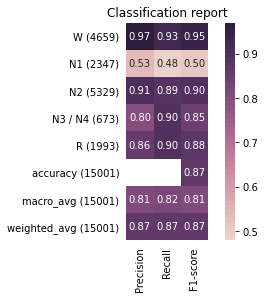
\includegraphics[width=.6\linewidth]{metrics/class_report.png} 
    \caption{Results: MASS training and MASS testing, 60 subjects - Classification report} 
    \label{fig:class_report} 
\end{figure}

\subsubsection{Balanced Accuracy}
Balanced accuracy is a metric that is often used of imbalanced classes problems since it takes into account the varied nature of the classes. 

In case of multiple classes, balanced accuracy is defined as the average of the recall for each class. In our example, and according to the classification report in Figure \ref{fig:class_report} we get:
\begin{align*}
   \texttt{balanced accuracy}= \frac{\sum_{i \in \{W, 1, 2, 3, R\}}\texttt{recall}_i}{5}= \frac{0.93+0.48+0.89+0.9+0.9}{5} \simeq 0.820.
\end{align*}
We can notice that there is a significant difference between the accuracy and the balanced accuracy in our example, which is due to the very low recall for the class N1.

\subsubsection{Cohen's kappa coefficient}
Cohen's kappa coefficient, denoted $\kappa$ is generally used to measure inter-rater reliability in the context of a binary classification, it can also be used to measure the performance by measuring the agreement between a true label and a predicted label. 

For a binary classification, we have the following:
\begin{align*}
    \kappa &= \frac{p_o-p_e}{1-p_e}, \\
    p_o &= \texttt{accuracy}, \\
    p_e &= \frac{(TP+FN)(TP+FP)}{S}+\frac{(TN+FP)(TN+FN)}{S}.
\end{align*}
where $p_o$ represents the relative observed agreement among raters (i.e. accuracy), and $p_e$ represents the hypothetic probability of chance agreement. 

For our example of multi-class classification, we get the following:
\begin{align*}
       \kappa = \frac{\sum_{i \in \{W, 1, 2, 3, R\}} M_{ii} \cdot S - \sum_{k \in \{W, 1, 2, 3, R\}} p_k \cdot t_k}{S^2 - \sum_{k \in \{W, 1, 2, 3, R\}} p_k \cdot t_k},
\end{align*}
and as $\sum_{k \in \{W, 1, 2, 3, R\}} p_k \cdot t_k = 18288880$, we get:
\begin{align*}
    \kappa &= \frac{7013\cdot8037-18288880}{8037^2-18288880} \simeq 0.822, 
\end{align*}
which is quite close to the score we obtained for the balanced accuracy but better takes into account both the recall and the precision of each class.

\newpage
\section{Results and Discussion}
In this section, we shall present and discuss our results for the various experiments we did. We will also discuss the limitations of our study and areas to explore for further works. 

\subsection{Results}
The results presented and discussed below correspond to the main experiment described in Section \ref{section:exp}, that is training the model with 48 subjects and testing it with 12 subjects coming from 2 different datasets. We compared MASS with both SleepPhysionet and our Clinical dataset. 

For each pair of datasets, we will present three different types of results: a table of scores (containing the balanced accuracy score in bold and Cohen's Kappa score in italics), a table of normalised confusion matrices (using the same standards as in Figure \ref{fig:conf_mat} and \ref{fig:norm_conf_mat} with the predicted labels on the horizontal axis and the true labels on the vertical axis), and a table of classification reports (containing the precision, the recall and the F1-score for each class).

\subsubsection{MASS and SleepPhysionet}
Let us first present the results when comparing MASS with SleepPhysionet. 

We obtain the following table of scores Table \ref{tab:scores_sp}. We notice a very important difference between the values on the diagonal which we did not really expect at first. It shows that our model performs much better on MASS than on SleepPhysionet in general. There are three possible reasons for this difference: the preprocessing steps are not very adapted, the algorithm was initially benchmarked using the MASS dataset, and our hyperparameters are not optimal for SleepPhysionet. A Parietal team member who consistently obtains a balanced accuracy around 0.76 on SleepPhysionet confirmed that our results are not as high as we could achieve.

We also notice that our model transfers much better from SleepPhysionet to MASS (0.560 of balanced accuracy) than from MASS to SleepPhysionet (0.487 of balanced accuracy), which is probably due to some specificity in the MASS dataset that we are unable to explain at this stage.

\begin{table}[!ht]
    \centering
    \begin{tabular}{|c||c|c|}
    \hline
    \diagbox{Training set}{Testing set} & MASS              & SleepPhysionet    \\ 
    \hline \hline
    \multirow{2}{*}{MASS}               & \textbf{0.802}    & \textbf{0.487}    \\ 
                                        & \textit{0.815}    & \textit{0.384}    \\ 
    \hline
    \multirow{2}{*}{SleepPhysionet}     & \textbf{0.560}    & \textbf{0.634}        \\  
                                        & \textit{0.488}    & \textit{0.618}        \\ 
    \hline
    \end{tabular}
    \caption{Table of results, comparing the datasets MASS and SleepPhysionet}
    \label{tab:scores_sp}
\end{table}

We can also compare the confusion matrices shown in Table \ref{tab:conf_mat_sp}. We immediately notice the low scores in the N1 column, showing that the model rarely predicts N1, without consistently predicting the same label instead of N1 as shown by the variety of scores in the N1 row, for amy pair of datasets.

\begin{table}[!ht]
    \centering
    \begin{tabular}{c|c|c|}
    \cline{2-3}
    & MASS              & SleepPhysionet    \\ 
    \hline
    \multicolumn{1}{|c|}{\rotatebox{90}{\centering MASS}}   & 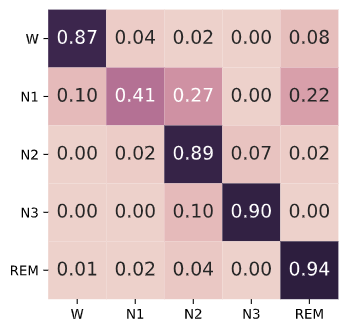
\includegraphics[width=0.45\linewidth]{confusion_matrix/mass-mass-4ch.png}    & 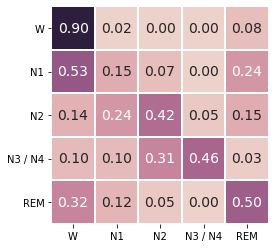
\includegraphics[width=0.45\linewidth]{confusion_matrix/mass-sp.png}     \\ 
    \hline
    \multicolumn{1}{|c|}{\rotatebox{90}{\centering SleepPhysionet}} & 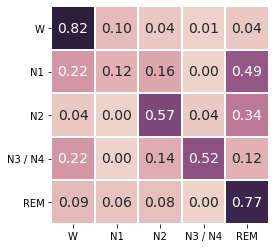
\includegraphics[width=0.45\linewidth]{confusion_matrix/sp-mass.png}    & 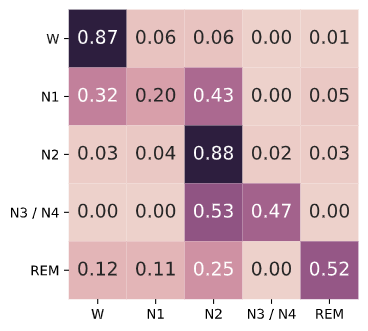
\includegraphics[width=0.45\linewidth]{confusion_matrix/sp-sp.png}        \\  
    \hline
    \end{tabular}
    \caption{Table of confusion matrices, comparing the datasets MASS and SleepPhysionet}
    \label{tab:conf_mat_sp}
\end{table}

We also present the classification reports in Table \ref{tab:class_report_sp}. Again, the N1 row stands out, and the sample count on the legend makes it quite clear that the N1 sleep stage is difficult to predict since it is rare. The MASS-MASS (trained on MASS and tested on MASS) classification report stands out thanks to its very high scores, emphasising once again the wide difference in terms of scores. We however notice in the MASS-MASS that the trade-off between precision and recall for N1 isn't optimal as the precision is quite high (0.58) compared to the recall (0.41). We notice that the difference between precision and recall is often important for other sleep stages and for other pairs of datasets as well.

\begin{table}[!ht]
    \centering
    \begin{tabular}{c|c|c|}
    \cline{2-3}
    & MASS              & SleepPhysionet    \\ 
    \hline
    \multicolumn{1}{|c|}{\rotatebox{90}{\centering MASS}}   & 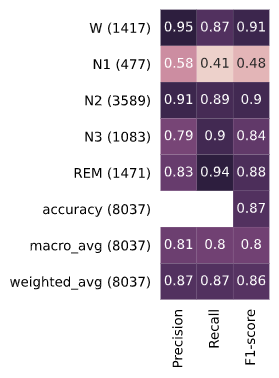
\includegraphics[width=0.4\linewidth]{classification_report/mass-mass-4ch.png}    & 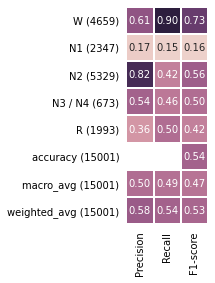
\includegraphics[width=0.4\linewidth]{classification_report/mass-sp.png}     \\ 
    \hline
    \multicolumn{1}{|c|}{\rotatebox{90}{\centering SleepPhysionet}} & 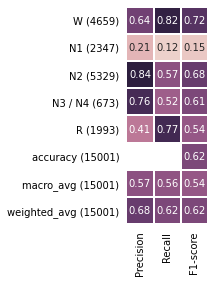
\includegraphics[width=0.4\linewidth]{classification_report/sp-mass.png}    & 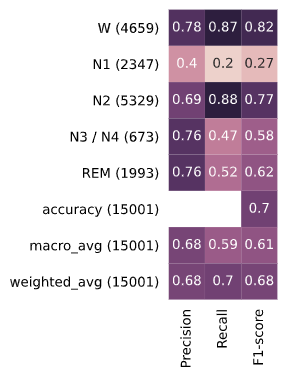
\includegraphics[width=0.4\linewidth]{classification_report/sp-sp.png}        \\  
    \hline
    \end{tabular}
    \caption{Table of classification reports, comparing the datasets MASS and SleepPhysionet}
    \label{tab:class_report_sp}
\end{table}

\subsubsection{MASS and Clinical}

We shall now present the results when comparing MASS with our Clinical dataset. 

\begin{table}[!ht]
    \centering
    \begin{tabular}{|c||c|c|}
    \hline
    \diagbox{Training set}{Testing set} & MASS              & Clinical          \\ 
    \hline \hline
    \multirow{2}{*}{MASS}               & \textbf{0.817}    & \textbf{0.390}    \\ 
                                        & \textit{0.822}    & \textit{0.287}    \\ 
    \hline
    \multirow{2}{*}{Clinical}           & \textbf{0.530}    & \textbf{0.635}    \\  
                                        & \textit{0.557}    & \textit{0.697}    \\ 
    \hline
    \end{tabular}
    \caption{Table of results, comparing the datasets MASS and Clinical}
    \label{tab:scores_clin}
\end{table}

We obtain the following table of scores Table \ref{tab:scores_clin}. In comparison to previous results, we notice an increase in the scores for MASS-MASS (0.817 compared to 0.802 in terms of balanced accuracy) which is due to the fact that we use more EEG channels when comparing MASS with Clinical than with SleepPhysionet. 

\begin{table}[ht!]
    \centering
    \begin{tabular}{c|c|c|}
    \cline{2-3}
    & MASS              & Clinical    \\ 
    \hline
    \multicolumn{1}{|c|}{\rotatebox{90}{\centering MASS}}   & 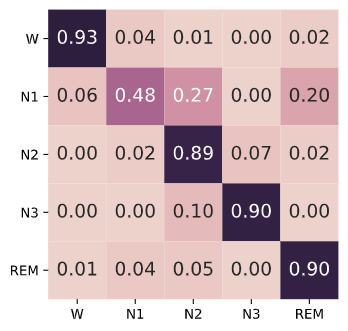
\includegraphics[width=0.45\linewidth]{confusion_matrix/mass-mass-9ch.png}    & 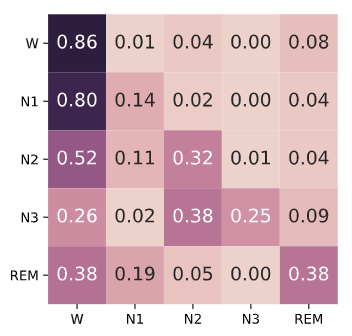
\includegraphics[width=0.45\linewidth]{confusion_matrix/mass-clin.png}     \\ 
    \hline
    \multicolumn{1}{|c|}{\rotatebox{90}{\centering Clinical}} & 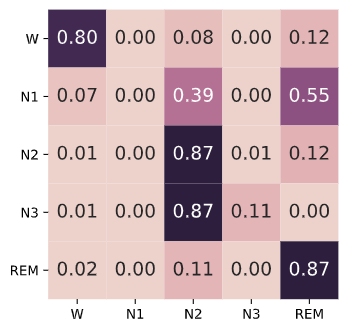
\includegraphics[width=0.45\linewidth]{confusion_matrix/clin-mass.png}    & 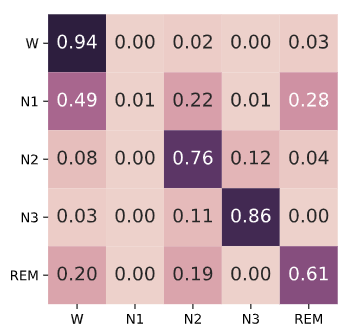
\includegraphics[width=0.45\linewidth]{confusion_matrix/clin-clin.png}        \\  
    \hline
    \end{tabular}
    \caption{Table of confusion matrices, comparing the datasets MASS and Clinical}
    \label{tab:conf_mat_clin}
\end{table}

Once again, we notice a very important difference between the values on the diagonal which shows unsurprisingly that our model performs much better on MASS than on our Clinical dataset.  We moreover notice that the model performs similarly on Clinical-Clinical (0.635 in balanced accuracy) and on SleepPhysionet-SleepPhysionet (0.634 in balanced accuracy). This may seem surprising at first as we could expect clinical data to be more noisy than SleepPhysionet but may be explained by the fact that we used more channels with the Clinical dataset. 

\begin{table}[ht!]
    \centering
    \begin{tabular}{c|c|c|}
    \cline{2-3}
    & MASS              & Clinical    \\ 
    \hline
    \multicolumn{1}{|c|}{\rotatebox{90}{\centering MASS}}   & 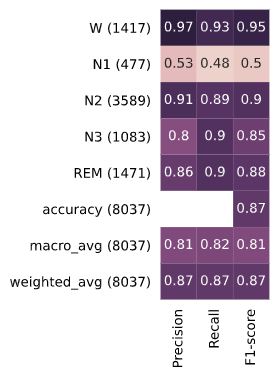
\includegraphics[width=0.4\linewidth]{classification_report/mass-mass-9ch.png}    & 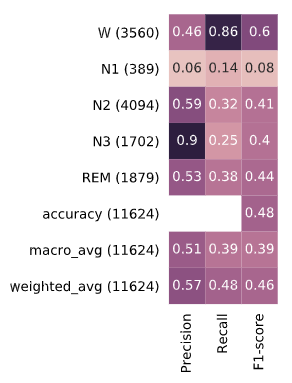
\includegraphics[width=0.4\linewidth]{classification_report/mass-clin.png}     \\ 
    \hline
    \multicolumn{1}{|c|}{\rotatebox{90}{\centering Clinical}} & 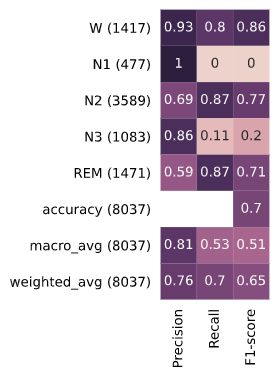
\includegraphics[width=0.4\linewidth]{classification_report/clin-mass.png}    & 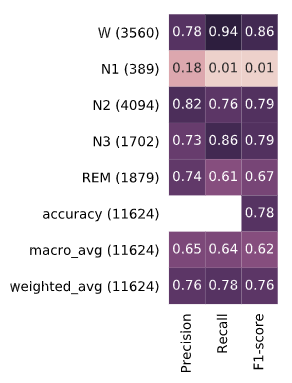
\includegraphics[width=0.4\linewidth]{classification_report/clin-clin.png}        \\  
    \hline
    \end{tabular}
    \caption{Table of classification reports, comparing the datasets MASS and Clinical}
    \label{tab:class_rep_clin}
\end{table}

In a similar manner as in our comparison between MASS and SleepPhysionet, we also notice that our model transfers much better from Clinical to MASS (0.530 of balanced accuracy) than from MASS to Clinical (0.390 of balanced accuracy). Again, this may due to some specificity in the MASS dataset.

In terms of confusion matrices, see Table \ref{tab:conf_mat_clin}, we notice a similar behaviour with regards to N1, this class is quite difficult to predict (as shown column-wise), and sample from this classs are not consistently predicted the same label (as shown row-wise). We further notice in Clinical-MASS (trained on Clinical and tested on MASS) that there are only 0 in the N1 column, showing that N1 was extremely rarely predicted. In that same confusion matrix, we notice that N2 is very often predicted. On the opposite, for MASS-Clinical, we notice that $W$ is very often predicted. It is however quite difficult to explain these differences at this stage.

We also present the classification reports in Table \ref{tab:class_rep_clin}. Again, the N1 row stands out due to its very low values. The MASS-MASS classification report stands out due to its very high values, emphasising once again the wide difference in terms of scores. It is however not very different compared to Clinical-Clinical except from the N1 row. This is a perfect example of the impact of a very low score in a rare class in terms of balanced accuracy. 

\subsection{Discussion}
Overall, we observe that even though this model performs quite well on MASS-MASS (trained on MASS and tested on MASS), it doesn't generalise quite as well on other datasets as shown in the results for SleepPhysionet-SleepPhysionet and Clinical-Clinical. These results, obtained when training and testing on the same dataset and appearing on the diagonals above, could surely be improved by tuning the hyperparameters of our model like the batch size, the number of epochs, the patience and the learning rate. 

These results also allow us to confirm that domain adaptation is one of the big challenges of sleep stage classification algorithm. We notice a very big difference with regards to all of the metrics evoked above in Section \ref{section:exp} when training and testing on different datasets. 

Throughout our study, we also had to handle different datasets, and we noticed that dealing with clinical datasets was quite challenging. There does not seem to exist a set of standard practices, that would provide doctors with precise guidelines, in terms of labelling of electrodes (some labels were in French whilst others were in English for example), annotations of sleep stages etc. Our clinical dataset also contains a majority of subjects who are suffering from sleeping disorders, which surely impacts their polysomnography data.

Through various side experiments for which we have not provided results here, we were able to observe other factors influencing the performance of our model. In particular, we can confirm that increasing the number of EEG channels included in the study can result in an increased performance (up to a point). And more importantly, using various modalities like adding EOG and EMG significantly improves the performance of this specific model. 

\subsection{Limitations and Further works}

It is important to keep in mind the fact that SleepPhysionet, MASS and our Clinical dataset do not use the same sleep stage scoring convention, as SleepPhysionet is scored according to the Rechtschaffen and Kales guidelines whilst SleepPhysionet and MASS are both scored according to the AASM manual. The main differences are: the existence of the $N4$ sleep stage in the Rechtschaffen and Kales rules, and the transition rules between different sleep stages. It could be interesting to score SleepPhysionet according to the AASM guidelines and to compare the performance and if the model would be able to generalise between MASS and SleepPhysionet any better. 

It would also be interesting to try to improve the model's architecture and to tune the hyperparameters to improve performance on SleepPhysionet-SleepPhysionet and Clinical-Clinical. We could also consider going as far as changing the architecture of the model to better predict data from datasets like Clinical and SleepPhysionet. We could also consider revising the pre-processing steps to make sure they are adapted to the various datasets.
We could go as far as studying the core differences in the raw data, in terms of noise for example, and to find methods to cope for these differences. 

\section{Conclusion and Acknowledgements}
I have greatly appreciated working on this project, studying machine learning in greater depth and getting to know more about the brain, sleep and electroencephalography. 

I would like to warmly thank Dr Alexandre Gramfort and Dr Olivier Pallanca for accompanying and guiding me throughout this project, giving me their insights and answering my questions. 

\newpage

\addcontentsline{toc}{section}{Code excerpts}
\section*{Code excerpts}
\begin{multicols}{2}
    \lstinputlisting[language=Python, caption=Implementation of the CNN in Pytorch]{code/sleep_stager_chambon.py}
    \lstinputlisting[language=Python, caption=BIDS conversion of Clinical]{code/clinical_to_bids_from_clean_annot.py}
\end{multicols}

\newpage 
\addcontentsline{toc}{section}{References}
\printbibliography

\addcontentsline{toc}{section}{Figures and Tables}
\listoffigures
\listoftables
\newpage

\end{document}
